\section{Comparison}
\label{sec:comparison}

% ANN vs. SNN
\acp{SNN} differ from normal \acp{ANN} in terms of their architecture and learning method.
Their inputs are 1-bit spike trains as opposed to 32- or 64-bit messages of \acp{ANN} \cite{SNN}.
The input of \acp{SNN} are streams of events which differs from the singular presentation of \acp{ANN} inputs \cite{ANN_SNN_conversion}.
Moreover, instead of backpropagation used for \acp{ANN}, many \ac{SNN} models have different learning rules to optimise their weight, 
such as \acfi{STDP} with exponential time dependence.

% original paper
\authorsSNN{} present an unsupervised approach to train a \ac{SNN} model \cite{SNN}.
However, there are other approaches to train \acp{SNN}, as well as opinions with regard to the biological plausibility of the methods used.


% STDP-like paper
The \ac{SNN} model presented by \authorsSTDPlike{} \cite{STDP_like} determines its output by 
choosing the class of the first neuron pool to reach the decision threshold with its accumulated sensory evidence.
The authors claim that the original method of using a majority vote of single threshold-based neuron activity is less biologically plausible.

Not only \authorsSTDPlike{}'s model \cite{STDP_like} but also \authorsSNN{}'s model \cite{SNN} use inhibition.

The \authorsSTDPlike{} point out that the classifier neurons will not recognize atypical digits (i.e. their stimulus) \cite{STDP_like}.
Therefore, the ability to generalize on new datasets depends on the inputs' similarity to the learned patterns.


% multi_scale_STDP paper
The model presented by both \authorsmultiScaleSTDP{} \cite{multi_scale_STDP} and \authorsSTDPvisFeat{} \cite{STDP_vis_feat} 
is designed to execute object recognition tasks in a biologically plausible manner.
It differs from the \authorsSNN{}'s model \cite{SNN} in multiple ways:

The first difference is the architecture \cite{multi_scale_STDP,STDP_vis_feat}.
%usage of a five-layer hierarchical network structure, consisting of alternating so-called simple cells $S_1, S_2$ and complex cells $C_1, C_2$.
%The simple cells employ intensity-to-latency conversion, i.e. the stronger a cell is stimulated the earlier it will fire \cite{STDP_vis_feat}.
%In a group of four simple cells, the cell with the earliest firing time inhibits the other cells and thus, creating winner-take-all inhibition \cite{multi_scale_STDP}.
%The spike omitted by the winner cell is then propagated asynchronously.
%It serves as input for the complex cells.
%Since there are fewer complex cells than simple ones, the complex cells propagate only the maximum, i.e. the earliest spike \cite{STDP_vis_feat}, of the input spikes.

%The second difference is the use of a classifier in the fifth layer to carry out the classification task 
The second difference is the use of a classifier to carry out the classification task 
instead of deciding on the class whose neurons have the highest average firing rate, 
as suggested by \authorsSNN{} \cite{SNN}.

Moreover, the model has a multi-scale form \cite{multi_scale_STDP}, i.e. the original image is scaled to different processing scales 
(100\%, 71\%, 50\%, 30\% and 25\%) and parallelly processed until 
all processing scales are combined in one of the layers.
%the fourth layer.

However, there are also similarities to \authorsSNN{}'s model \cite{SNN}:
%The $C_1$ to $S_2$ synaptic connections are trained using \ac{STDP} \cite{multi_scale_STDP,STDP_vis_feat}.
The synaptic connections are trained using \ac{STDP} \cite{multi_scale_STDP,STDP_vis_feat}.
Yet, the time difference between the presynaptic and postsynaptic spike is only used to determine the sign of the modification of the synaptic weight 
but is not relevant for the amount of weight change \cite{STDP_vis_feat}.

Both \authorsmultiScaleSTDP{}'s model \cite{multi_scale_STDP} and \authorsSNN{}'s model \cite{SNN} use inhibition and thus, 
create competition and consequently ensure all neurons learn a distinct pattern to cover the whole variability of inputs \cite{STDP_vis_feat}.
%
%\authorsmultiScaleSTDP{}'s model \cite{multi_scale_STDP} is trained and evaluated on the ETH-80 and 3D-Object datasets \cite{multi_scale_STDP}, which contain objects with large deviations.
%The data is converted to grayscale values.
%A \ac{RDM} is used to determine whether the quality of the model is good enough to provide a representation of objects which have a high inter-category dissimilarity and a low intra-category dissimilarity.
%The result of the \ac{RDM} in \autoref{fig:RDM_SNN} suggests that the model is able to distinguish between feature values of different categories.
%The authors include a \ac{RDM} of a non-\ac{SNN} model performing considerably worse.
%
%\begin{figure}[htbp]
%    \center
%    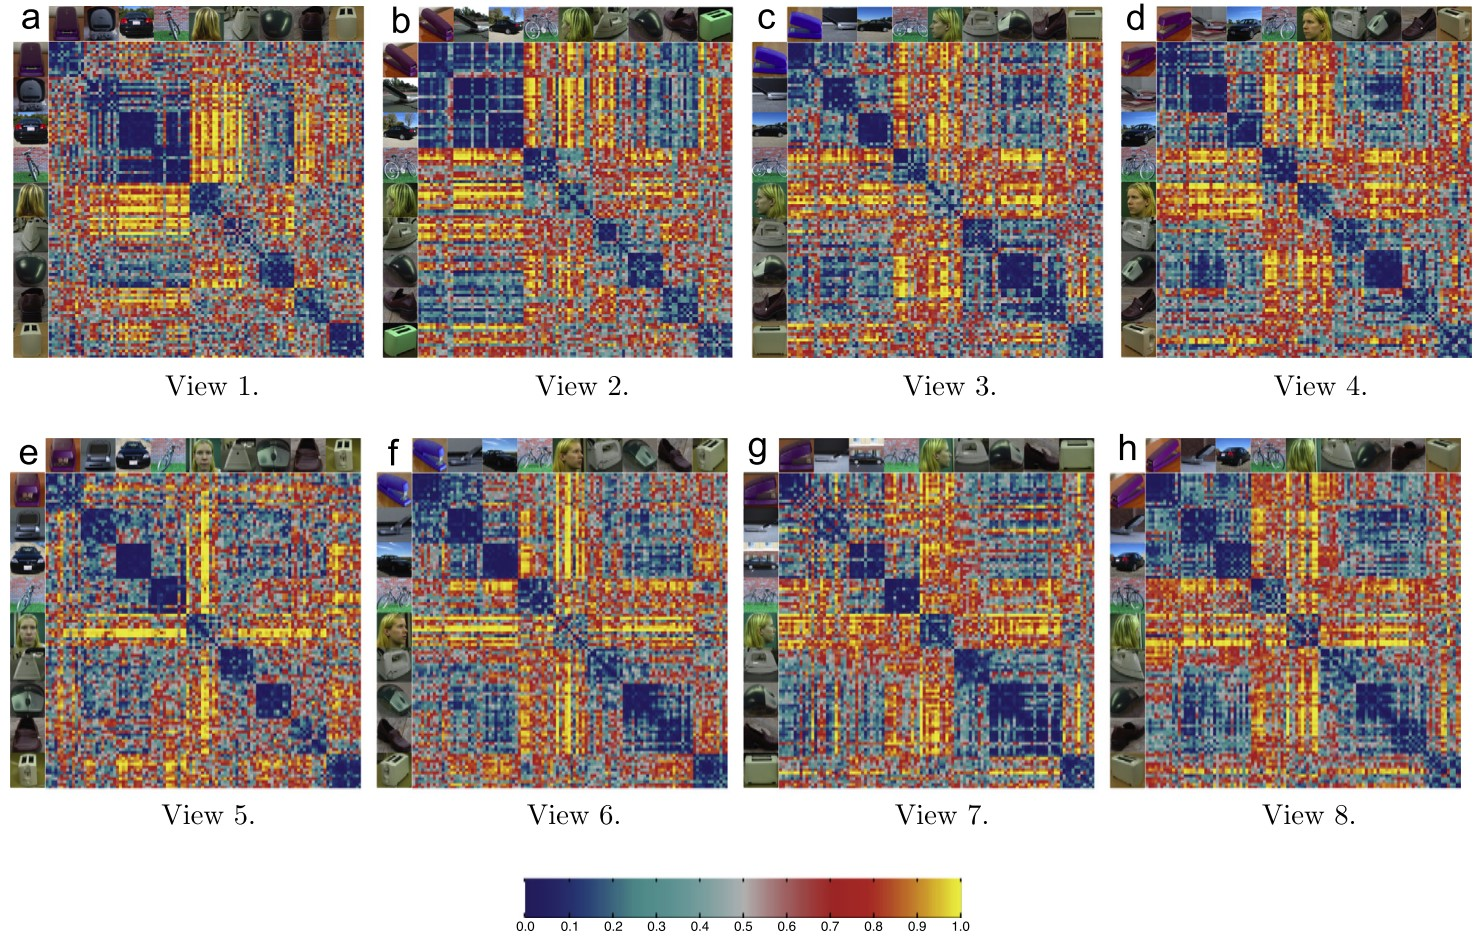
\includegraphics[width=0.7\textwidth]{pictures/inter_intra_category_dissimilarity.jpg}
%    \caption{\acp{RDM} of object representations of different image stimuli for different views from \authorsmultiScaleSTDP{}'s paper \cite{multi_scale_STDP}.
%    A sample image for each category is placed next to the rows and columns.
%    Intra-class dissimilarity is low, and inter-class dissimilarity is high.}
%    \label{fig:RDM_SNN}
%\end{figure}
%
%The model becomes selective to the prominently present patterns in the input and generates fast responses \cite{STDP_vis_feat}.
The multi-scale \ac{SNN} is well suited for object recognition tasks consisting of few classes and many viewpoints \cite{multi_scale_STDP}.
The authors admit that processing time for many classes would greatly increase.

% triplet-based STDP paper
\authorsSTDPtriplet{} \cite{STDP_triplet} claim that classical pair based \ac{STDP} models 
are not able to explain synaptic changes caused by triplets or quadruplets of spikes.